This section provides some information on various
implementation details for the Jikes\TMweb{} RVM runtime system.

\subsection{Object Model}\label{sssec:objects}
\index{object model}

An {\em object model} dictates how to represent objects in storage;
the best object model will maximize efficiency of frequent language
operations while minimizing storage overhead. \jrvm's
object model is defined by 
\xlink{{\tt VM\_ObjectModel.java}}{\VMObjectModelURL}.
The \jrvm object model underwent major changes between versions
2.3.3 and 2.3.4 of the system.  In particular, in 2.3.3 and before a 
``reverse scalar'' object model was used in which scalars and arrays
were layed out in different directions in memory to optimize null
pointer checks on AIX. 

\paragraph{Overview}
Values in the Java\TMweb{} programming language are either {\em
primitive} ({\it e.g.}\ {\tt int}, {\tt double}, etc.)  or they are {\em
references} (that is, pointers) to objects.  Objects are either {\em
arrays} having elements or {\em scalar objects} having fields.
Objects are logically composed of two primary sections: an object
header (described in more detail below) and the object's instance
fields (or array elements). 

The following non-functional requirements govern the Jikes RVM object model:
\begin{itemize}
\item
instance field and array accesses should be as fast as possible,
\item
null-pointer checks should be performed by the hardware if possible, 
\item
method dispatch and other frequent runtime services should be fast,
\item
other (less frequent) Java operations should not be prohibitively
slow, and
\item
per-object storage overhead (ie object header size) should be as small
as possible.
\end{itemize}

\index{field access}
\index{array access}
Assuming the reference to an object resides in a register, compiled
code can access the object's fields at a fixed displacement in a
single instruction.  To facilitate array access, the reference to an
array points to the first (zeroth) element of an array and the
remaining elements are laid out in ascending order.  The number of
elements in an array, its {\em length}, resides just before its first
element. Thus, compiled code can access array elements via base +
scaled index addressing.

The Java programming language requires that an attempt to access an
object through a {\tt null} object reference generates a
\IndexTexttt{NullPointerException}.  In Jikes RVM, references are
machine addresses, and {\tt null} is represented by address $0$.  
On Linux, accesses to both very low and very high memory can be
trapped by the hardware, thus all null checks can be made implicit.
However, the AIX\TMweb{} operating system permits loads from low
memory, but accesses to very high memory (at small {\em negative}
offsets from a null pointer) normally cause hardware 
interrupts. Therefore on AIX only a subset of pointer dereferences can
be protected by an implicit null check. 

\paragraph{Object Header}
\index{object header}
Logically, every object header contains the following components:
\begin{description}
%
\index{TIB}
\index{superclass}
\index{interfaces}
\index{virtual methods}
\begin{Label}{TIB}
\item[TIB Pointer] The TIB (Type Information Block) holds information that
applies to all objects of a type.  The structure of the TIB is defined by 
\xlink{{\tt VM\_TIBLayoutConstants.java}}{\VMTIBLayoutConstantsURL}.
A TIB includes the virtual method table, a pointer to an object
representing the type, and pointers to a few data structures to
facilitate efficient interface invocation and dynamic type checking.
\end{Label}
%
\index{hashing}
\item[Default Hash Code] Each Java object has a default hash code.
%
\index{locking}
\item[Lock] Each Java object has an associated lock state.  This could be a
pointer to a lock object or a direct representation of the lock.
%
\item[Array Length] Every array object provides a {\em length} field
that contains the length (number of elements) of the array.
%
\item[Garbage Collection Information] Each Java object has associated
information used by the memory management system.  Usually this consists of one
or two mark bits, but this could also include some combination of a reference
count, forwarding pointer, etc.
%
\item[Misc Fields] In experimental configurations, the object header
can be expanded to add additional fields to every object, typically to
support profiling. 
\end{description}

An implementation of this abstract header is defined by three files: 
\xlink{{\tt VM\_JavaHeader.java}}{\VMJavaHeaderURL}, which supports
\link{TIB}{TIB} access, default hash codes, and locking; 
\xlink{{\tt VM\_AllocatorHeader.java}}{\VMAllocatorHeaderURL}, which
supports garbage collection information; 
and 
\xlink{{\tt VM\_MiscHeader.java}}{\VMMiscHeaderURL}, which supports
adding additional fields to all objects. 

As of Jikes RVM 2.2.1, the system supports only one implementation
\xlink{{\tt VM\_JavaHeader.java}}{\VMJavaHeaderURL}; 
defining a two-word header for scalar objects.  The source tree includes
three other object models which are currently unsupported, but may be
resurrected in a future release.

\subsection{Methods and Fields}\label{sssec:methods}
\index{methods}
\index{JTOC}
\index{TIB}
\begin{Label}{JTOC}
A compiled method body is an array of machine instructions (stored as
{\tt int}s on PowerPC\TMweb{} and {\tt byte}s on x86-32). 
The {\em Jikes RVM Table of Contents} (JTOC),
stores pointers to static fields and methods.  However, 
pointers for instance fields and virtual methods are stored in the receiver 
class's \link{TIB}{TIB}.  Consequently, the dispatch mechanism differs
between static methods and instance methods.
\end{Label}

\paragraph{The JTOC}
\index{JTOC}
\begin{figure}[htb]
\begin{gif}{jtoc}
\vbox{
\hbox{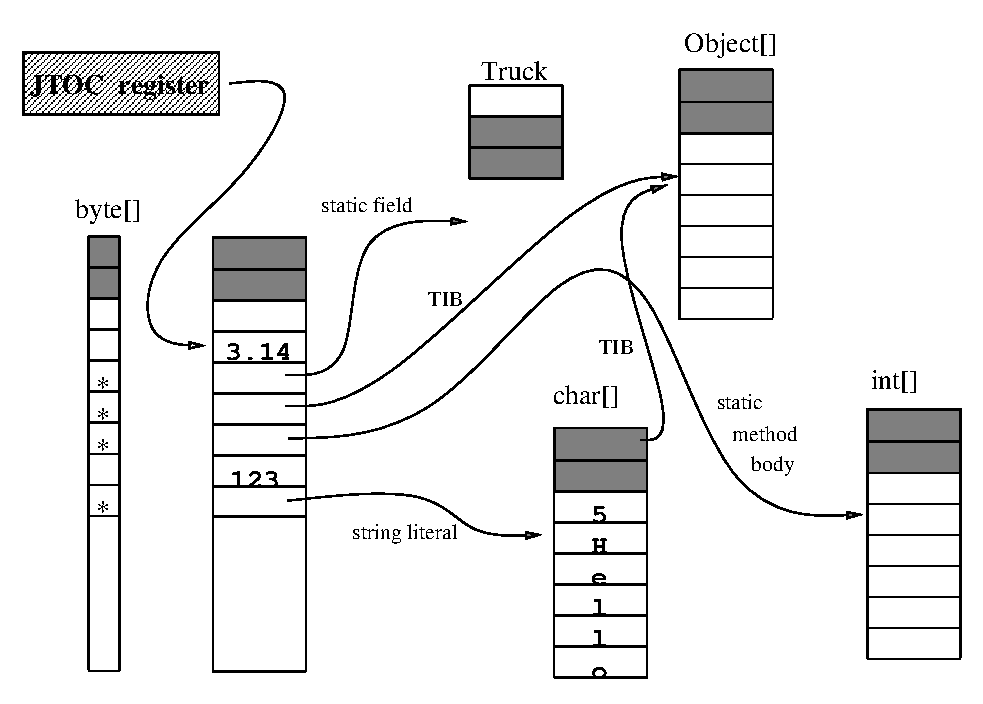
\psfig{file=jtoc.ps,height=3.5in}}
}\hfil
\end{gif}
\caption{The Jikes RVM Table Of Contents and other objects.}
\label{fig:jtoc}
\end{figure}
\index{literals}
\index{constants}
\index{dynamic type checking}
The JTOC holds pointers to 
each of Jikes\TMweb{} RVM's global data structures, as well as
literals, numeric constants and references to \texttt{String} constants.
The JTOC also
contains references to the \link{TIB}{TIB} for each class in the system.  
Since these 
structures can have many types and the JTOC is declared to be an array of 
{\tt int}s,  
Jikes RVM uses a descriptor array, co-indexed with the JTOC, 
to identify the entries containing references.
The JTOC
is depicted \link*{in this figure}[in figure~\Ref, on page~\Pageref{}]{fig:jtoc}.  

\paragraph{Virtual Methods}
\index{virtual methods}
A \link{TIB}{TIB} contains pointers to the compiled method 
bodies (executable code) for the virtual methods of its class. 
Thus, the \link{TIB}{TIB} serves as Jikes RVM's virtual method table.
A virtual method dispatch entails loading the \link{TIB}{TIB} pointer from 
the object reference, loading the address of the method
body at a given offset off the \link{TIB}{TIB} pointer, and making an indirect
branch and link to it.

\paragraph{Static Fields and Methods} 
\index{static methods}
Static fields and pointers to static method bodies are stored in the \link{JTOC}{JTOC}. 
Static method dispatch is simpler than virtual dispatch, since 
a well-known \link{JTOC}{JTOC} entry method holds the address of the compiled method
body. 

\paragraph{Lazy Method Compilation}\label{par:lazy}
\index{lazy method compilation}
\index{deferred compilation}
\index{lazy method invocation stub}
Method slots in a \link{TIB}{TIB} or the \link{JTOC}{JTOC} may hold either
a pointer to the compiled code, 
or a pointer to the compiled code of the {\em lazy method invocation stub}.
When invoked, the lazy method invocation stub compiles the 
method, installs a pointer to the compiled code in the appropriate
\link{TIB}{TIB} or the \link{JTOC}{JTOC} slot, then 
jumps to the start of the compiled code. 

\paragraph{Interface Methods}
\index{interface methods}
\index{IMT}
\index{conflict resolution stub}
Regardless of whether or not a virtual method is overridden,
virtual method dispatch is still simple since the method will occupy 
the same \link{TIB}{TIB} offset its defining class and in every sub-class.
However, a method invoked through an {\tt invokeinterface} call rather than
an {\tt invokevirtual call}, will not occupy the same \link{TIB}{TIB} offset in every class that 
implements its interface.  This complicates dispatch for {\tt
invokeinterface}.

\index{Interface Method Table (IMT)}%
\index{IMT: Interface Method Table}%
The simplest, and least efficient way, of locating an interface method 
is to search all the virtual method entries in the \link{TIB}{TIB} finding a match.
Instead, Jikes RVM uses an {\em Interface Method Table} (IMT) which resembles
a virtual method table for interface methods. Any method that could be an interface method has 
a fixed offset into the IMT just as with the \link{TIB}{TIB}. However, unlike in the \link{TIB}{TIB}, two different methods may
share the same offset into the IMT.\@ In this case, a
\index{conflict resolution stub}{\em conflict resolution
stub} is inserted in the IMT.\@ Conflict resolution stubs are
custom-generated machine code sequences that test the value of a
hidden parameter to dispatch to the desired interface method.
For more details, see
\xlink{{\tt VM\-\_In\-ter\-face\-In\-vo\-ca\-tion\-.java}}{\VMInterfaceInvocationURL}.

\subsection{VM Conventions}

\subsubsection{AIX/PowerPC VM Conventions}
\label{aix-conventions}

\index{stack conventions: AIX/PowerPC}
\index{register conventions: AIX/PowerPC}
\index{calling conventions: AIX/PowerPC}

This section describes register, stack, and calling conventions that apply to 
Jikes RVM on AIX\-/\-Pow\-er\-PC\TMweb{}.

Stackframe layout and calling conventions may evolve as our understanding
of Jikes RVM's performance improves.  Where possible, API's should be used
to protect code against such changes.  In particular, we may move to
the AIX\TMweb{} conventions at a later date.  Where code differs from the AIX
conventions, it should be marked with a comment to that effect containing
the string ``\texttt{AIX}''.

%\noindent{\bf Register conventions}
\paragraph{Register conventions}

Registers (general purpose, gp, and floating point, fp) can be roughly
categorized into four types:

\begin{description}
\item[Scratch]
     Needed for method prologue/epilogue.  Can be used by compiler between
     calls.

\item[Dedicated]
     Reserved registers with known contents:
\begin{description}
\item[\link{JTOC}{JTOC} - Jikes RVM Table Of Contents]
        Globally accessible data: constants, static fields and methods.

\item[FP - Frame Pointer]
        Current stack frame (thread specific).

\item[PR - Processor register]
        An object representing the current virtual processor (the one
        executing on the CPU containing these registers).  A field in
        this object contains a reference to the object representing
        the {\tt VM\_Thread} being executed.
\end{description}

\item[Volatile (``caller save'', or ``parameter'')]
     Like scratch registers, these can be used by the compiler as
     temporaries, but they are not preserved across calls.  Volatile
     registers differ from scratch registers in that volatiles
     can be used to pass parameters and result(s) to and from
     methods.

\item[Nonvolatile (``callee save'', or ``preserved'')]
     These can be used (and are preserved across calls), but they must be
     saved on method entry and restored at method exit.  Highest numbered
     registers are to be used first.  (At least initially, nonvolatile
     registers will not be used to pass parameters.)

\item[Condition Register's 4-bit fields]
We follow the AIX conventions to minimize cost in JNI transitions
between C and Java code. 
\begin{description}
\item[CR0, CR1, CR5, CR6, CR7] volatile
\item[CR2, CR3, CR4] non-volatile
\end{description}
The baseline compiler only uses CR0.  The opt compiler allocates CR0,
CR1, CR5 and CR6 and reserves CR7 for use in yieldpoints.  None of the
compilers use CR2, CR3, or CR4 to avoid saving/restoring condition
registers when doing a JNI transition from C to Java code. 
\end{description}


%\noindent{\bf Stack conventions}
\paragraph{Stack conventions}

Stacks grow from high memory to low memory.
The layout of the stackframe appears in a block comment in
\texorhtml{\texttt{\$RVM\_\-ROOT/\-rvm/\-src/\-vm/\-arch/\-powerpc/\-VM\_\-StackframeLay\-outCon\-stants.java}}{\xlink{\texttt{\$RVM\_\-ROOT/\-rvm/\-src/\-vm/\-arch/\-powerpc/\-VM\_\-StackframeLay\-outCon\-stants.java}}{\PPCStackframeLayoutURL}}.

%\noindent{\bf Calling Conventions}
\paragraph{Calling Conventions}

\begin{description}
\item[Parameters]

    All parameters (that fit) are passed in VOLATILE registers.  Object
    reference and int parameters (or results) consume one GP register; long
    parameters, two gp registers (low-order half in the first);  float and
    double parameters, one fp register.  Parameters are 
    assigned to registers
    starting with the lowest volatile register through the highest volatile
    register of the required kind (gp or fp).

    Any additional parameters are passed on the stack in a parameter spill
    area of the caller's stack frame.  The first spilled parameter occupies
    the lowest memory slot.  Slots are filled in the order that parameters
    are spilled.

    An int, or object reference, result is returned in the first volatile
    gp register; a float or double result is returned in the first volatile
    fp register; a long result is returned in the first two volatile gp
    registers (low-order half in the first);

\item[Method prologue responsibilities] (some of these can be omitted for leaf
  methods):

\begin{enumerate}
\item Execute a stackoverflow check, and grow the thread stack if necessary.

\item Save the caller's next instruction pointer (callee's return address,
       from the Link Register).

\item Save any nonvolatile floating-point registers used by callee.

\item Save any nonvolatile general-purpose registers used by callee.

\item Store and update the frame pointer FP.\@

\item Store callee's compiled method ID 

\item Check to see if the Java\TMweb{} thread must yield the {\tt VM\_Processor}
(and yield if threadswitch was requested). 
\end{enumerate}

\item[Method epilogue responsibilities] (some of these can be
ommitted for leaf methods):

\begin{enumerate}
\item Restore FP to point to caller's stack frame.

\item Restore any nonvolatile general-purpose registers used by callee.

\item Restore any nonvolatile floating-point registers used by callee.

\item Branch to the return address in caller.
\end{enumerate}
\end{description}

\subsubsection{Linux/x86-32 VM Conventions} \label{lintel-conventions}
\index{stack conventions: Linux/x86-32}
\index{register conventions: Linux/x86-32}
\index{calling conventions: Linux/x86-32}

This section describes register, stack, and calling conventions that
apply to Jikes RVM on Li\-nux\Rweb{}\-/x86-32.  

%\noindent{\bf Register conventions}
\paragraph{Register conventions}

\begin{description}
\item[EAX]
    First GPR parameter register, first GPR result value (high-order part
    of a long result), otherwise volatile (caller-save).

\item[ECX]
    Scratch.

\item[EDX]
    Second GPR parameter register, second GPR result value (low-order part
    of a long result), otherwise volatile (caller-save).

\item[EBX]
    Nonvolatile.

\item[ESP]
    Stack pointer.

\item[EBP]
    Nonvolatile.

\item[ESI]
    Processor register, reference to the VM\_Processor object for the current
    virtual processor.

\item[EDI]
    Nonvolatile.  (used to hold \link{JTOC}{JTOC} in baseline compiled code)

\end{description}

%\noindent{\bf Stack conventions}
\paragraph{Stack conventions}

Stacks grow from high memory to low memory.
The layout of the stackframe appears in a block comment in
\xlink{{\tt
\$RVM\_\-ROOT/\-rvm/\-src/\-vm/\-arch/\-in\-tel/\-VM\_\-Stack\-frame\-Lay\-out\-Con\-stants.java}}
{\LintelStackframeLayoutURL}.

%\noindent{\bf Calling Conventions}
\paragraph{Calling Conventions}

\begin{description}
\item[At the beginning of callee's prologue]
The first two areas of the callee's stackframe (see above) have been
     established.  ESP points to caller's return address.
     Parameters from caller to callee are as mandated by 
\xlink{{\tt
\$RVM\_\-ROOT/\-rvm/\-src/\-vm/\-arch/\-in\-tel/\-VM\_\-Re\-gis\-terCon\-stants.java}}
{\LintelRegisterConstantsURL}.

\item[After callee's epilogue]
     Callee's stackframe has been removed.  ESP points to the word above where
     callee's frame was.  The framePointer field
     of the VM\_Processor object pointed to by ESI points to A's
     frame.  If B returns a floating-point result, this is at
     the top of the fp register stack.  If B returns a long, the
     low-order word is in EAX and the high-order word is in EDX.\@
     Otherwise, if B has a result, it is in EAX.\@

\end{description}

\subsubsection{OS~X VM Conventions}
\index{calling conventions: OS X/PowerPC}

\paragraph{Calling Conventions}

\newcommand{\OSXCallingConventionsURL}{http:\-//\-de\-vel\-op\-er.ap\-ple.com/\-do\-cu\-men\-ta\-tion\-/\-De\-ve\-lo\-per\-Tools\-/\-Con\-cep\-tu\-al\-/\-Mach\-O\-Run\-time\-/\-Mach\-O\-Run\-time\-.pdf}
The calling conventions we use for OS~X are the same as those listed
at:
\begin{example}
\xlink{\texttt{\OSXCallingConventionsURL}}{\OSXCallingConventionsURL}
\end{example}
They're similar to the Linux PowerPC calling conventions.  One
major difference is how the two operating systems handle the case of
a \texttt{long} parameter when you only have a single parameter register left.


\subsection{Class Loading} \label{sssec:classLoading}
\index{class loading}

Jikes\TMweb{} RVM implements the Java\TMweb{} programming
language's dynamic class loading.  While a class is being loaded it can
be in one of six states. These are:
\begin{description}
\item[vacant] The class is in the process of being loaded.
\item[loaded] the class's bytecode file has been read and parsed successfully.
\item[resolved] the superclass of this class has been loaded and resolved and
the offsets (whether in the object itself, the \link{JTOC}{JTOC}, or the class's
\link{TIB}{TIB}) of its fields and methods have been calculated.
\item[instantiated] the superclass has been instantiated and pointers to the
compiled methods have been inserted into the \link{JTOC}{JTOC} (for static methods) and the
\link{TIB}{TIB} (for virtual methods).
\item[initializing] the superclass has been initialized and the class
initializer is being run.
\item[initialized] the superclass has been initialized and the class
initializer has been run.
\end{description}

The class passes through these states in the following fashion.

\paragraph{Vacant}
The 
\xlink{{\tt VM\_Class}}{\VMClassURL} 
object for this class has been created and registered and is in the
process of being loaded.

\paragraph{Loaded} 
\index{constant pool}
In this state the class file has been read and parsed.  The constant
pool has been constructed. The declared methods and fields of the
class have been loaded.  Loading a method or field consists of reading
its modifiers and attributes. The class's superclass (if any) and
superinterfaces have been loaded as well.

\paragraph{Resolved}
In this state the superclass and superinterfaces of this class have
been resolved as well.  A list of the virtual methods and instance fields
of this class, including the methods and fields inherited from its
superclass has been constructed and the offsets for the instance
fields have been calculated.  Space has been allocated in the \link{JTOC}{JTOC} for
all static fields of the class and for static method pointers and the
appropriate offsets calculated.  The \link{TIB}{TIB} has been initialized and
offsets for the virtual methods have been calculated.

\paragraph{Instantiated}
In this state the superclass has been instantiated.  The
slots in the \link{TIB}{TIB} are filled in with pointers to compiled code or \link{lazy
compilation stubs for
the virtual methods}[.  (See Paragraph~\Ref{} on page~\Pageref.)]{par:lazy}  The slots in the \link{JTOC}{JTOC} are filled in with
pointers to compiled code or lazy compilation stubs for the static methods.

\paragraph{Initializing} 
\index{class initializer}
In this state the superclass has been initialized. The class
initializer is being run. 

\paragraph{Initialized} 
\index{class initializer}
In this state the superclass has been initialized.  The class initializer has 
been run. 

\subsection{Thread System}\label{sec:threads}

This section provides some explanation of how Java\TMweb{} threads are
scheduled and synchronized by Jikes\TMweb{} RVM.\@

\index{threads}
\index{scheduling}
\index{locking}

\label{threads:single-virtual-processor}All Java threads (application threads, garbage collector threads, {\em
etc.})  derive from 
\xlink{{\tt VM\_Thread}}{\VMThreadURL}.  
These threads are multiplexed onto
one or more virtual processors (see 
\xlink{{\tt VM\_Processor}}{\VMProcessorURL}).  Normally, the
number of Jikes RVM virtual processors to use is a command line argument
({\it e.g.}\ {\tt -X:processors=4}) Generally, there should be one Jikes RVM
virtual processor for each CPU on an SMP.\@  Additional virtual
processors may be created to handle threads executing non-Java code
through the Java JNI.\@  Multiple virtual processors require a working
pThread library, each virtual processor being bound to a pThread.  It
is possible to build a system that only uses one virtual processor by
setting the preprocessor directive 
\varName{RVM\_\-FOR\_\-SIN\-GLE\_\-VIR\-TU\-AL\_\-PRO\-CES\-SOR} to 1.  This may give a minor
performance benefit on uniprocessors. See the configuration file
{\tt BaseBaseCopyMSUP} for examples of
using this preprocessor directive.

Threads that are not executing are either placed on thead queues
(deriving from 
\xlink{\texttt{VM\_\-Ab\-stract\-Thread\-Queue}}{\VMAbstractThreadQueueURL}
) or are proxied (see below).
Thread queues are either global or (virtual) processor local.  The
latter do not require synchronized access but global queues do.
Unfortunately, we did not see how to use Java monitors to provide
this synchronization.  (In part, because it is needed to implement
monitors, see below.)  Instead this low-level synchronization is
provided by 
\xlink{{\tt VM\_\-Pro\-ces\-sor\-Lock}}{\VMProcessorLockURL}s.

Transferring execution from one thread (A) to another (B) is a complex
operation negotiated by the {\tt yield} and {\tt morph} methods of
VM\_Thread and the {\tt dispatch} method of VM\_Processor.  {\tt
yield} places A on an indicated queue (releasing the lock on the
queue, if it is global).  {\tt morph} does some additional
housekeeping and transfers control to {\tt dispatch} which selects the
next thread to execute. Dispatch then invokes {\tt
VM\_Ma\-gic.thread\-Switch} to save the hardware context of A and restore
the hardware context of B.\@  It now appears as if B's previous call to
{\tt dispatch} has just returned and it continues executing. While
dispatching is proceeding (from the time A is enqueued until B's
hardware context is restored), the {\tt be\-ing\-Dis\-patched} field of A is
set to prevent it from being scheduled for execution on some other
virtual processor while it is still executing in {\tt morph } or {\tt
dispatch}. 

Beginning with version 2.0.1, Jikes RVM has a simple load balancing
mechanism. Every once in a while, a thread will move from one virtual
processor to the next.  Such movement happens when a thread is
interrupted by a timer tick (or garbage collection) or when it comes
off a global queue (such as, the queues waiting for a heavy-weight
lock, see \xlink{{\tt VM\_Lock}}{\VMLockURL}).  Such migration will be
inhibited if the thread is the last (non-idle) executable thread on
its current virtual processor.  

If a virtual processor has no other executable thread, its idle thread
runs.  This thread posts a request for work and then busy-waits for a
short time (currently 0.001 seconds).  If no work arrives in that
period, the virtual processor surrenders the rest of its time slice
back to the operating system.  If another virtual processor notices
that this one needs work, it will tranfer an extra runnable thread (if
it has one) to this processor.  When work arrives, the idle thread
yields to an idle queue, and the recently transferred thread begins
execution.

Currently, Jikes RVM has no priority mechanism, that is, all threads run at
the same priority.

If Jikes RVM detects that a thread is stuck executing native code (JNI)
for a long time, it temporarily prevents it from returning to Java code and
creates a new pThread (or recycles one previously created for this 
purpose) and transfers the stuck thread's virtual processor to the
new pThread.  When the stuck thread returns to Java code, the pThread
executing it is deactivated and added to a pool of available pThreads.
Currently, this mechanism does not work on Linux and is disabled there.

Jikes RVM uses a light-weight locking scheme to implement Java monitors (see
\xlink{{\tt VM\_Lock}}{\VMLockURL} and 
\xlink{{\tt VM\_\-Thin\-Lock}}{\VMThinLockURL}). The exact details of the
locking scheme are dependent on which variant of 
\xlink{{\tt VM\_\-Ja\-va\-Hea\-der.java}}{\VMJavaHeaderURL} is selected at
system build time.  If an object instance has a light weight lock,
then some bits in the object header are used for locking.  
If the top bit is set, the remainder of the bits 
are an index into an array of heavy-weight locks.
Otherwise, if the object is locked, these bits contain the id of the
thread that holds the lock and a count of how many times it is held.
If a thread tries to lock an object locked with a light-weight lock by
another thread, it can spin, yield, or inflate the lock.  Spinning is
probably a bad idea.  The number of times to yield before inflating is
a matter open for investigation (as are a number of locking
issues, see {\tt VM\_Lock}).  Heavy-weight locks contain an {\tt
enteringQueue} for threads trying to acquire the lock.

A similar mechanism is used to implement Java wait/notification
semantics.  Heavy-weight locks contain a {\tt waitingQueue} for
threads blocked at a Java {\tt wait}.  When a {\tt notify} is
received, a thread is taken from this queue and transferred to a ready
queue.  Priority {\tt wakeupQueue}s are used to implement Java sleep
semantics.  Logically, Java timed-wait semantics entail placing a
thread on both a {\tt waitingQueue} and a {\tt wakeupQueue}.  However, our
implementation only allows a thread to be on one thread queue at
a time.  To accommodate timed-waits, both {\tt wai\-ting\-Queue}s and
{\tt wake\-up\-Queue}s are queues of {\em proxies} rather than threads.
A \xlink{{\tt VM\_Proxy}}{\VMProxyURL} can represent the same thread
on more than one proxy queue.


\subsection{VM Callbacks}\label{sssec:callbacks}

\index{callbacks}

Jikes\TMweb{} RVM provides callbacks for many runtime events of
interest to the Jikes RVM 
programmer, such as classloading, VM boot image creation, and VM exit.  The
callbacks allow arbitrary code to be executed on any of the supported events.

The callbacks are accessed through the nested interfaces defined in the 
\xlink{{\tt VM\_\-Call\-backs}}{\VMCallbacksURL} 
class.  There is one interface per event type.  To be notified
of an event, register an instance of a class that implements the corresponding
interface with {\tt VM\_Callbacks} by calling the corresponding {\tt add...()}
method.  For example, to be notified \link{when a class is instantiated}[ (see section~\Ref)]{sssec:classLoading}, first implement the {\tt
VM\_Callbacks.ClassInstantiatedMonitor} interface, and then call {\tt
VM\_\-Call\-backs.add\-Class\-In\-stan\-ti\-a\-ted\-Mon\-i\-tor()} with an instance of your class.
When any class is instantiated, the {\tt notifyClassInstantiated} method in
your instance will be invoked.

\xlink{Jikes RVM supports callbacks for a number of events}[; see 
{\tt VM\_Callbacks} for the list of currently
supported callbacks]{\VMCallbacksURL}.

The appropriate interface names can be obtained by appending ``Monitor'' to the
event names (e.g. the interface to implement for the {\tt MethodOverride} event
is {\tt VM\_\-Call\-backs.Me\-thod\-Ov\-er\-ride\-Mo\-ni\-tor}).  Likewise, the method to
register the callback is ``add'', followed by the name of the interface (e.g.
the register method for the above interface is {\tt
VM\_\-Call\-backs.add\-Me\-thod\-O\-ver\-ride\-Mon\-i\-tor()}).

Since the events for which callbacks are available are internal to the VM,
there are naturally some limitations on the behavior of the callback code.  For
example, as soon as the exit callback is invoked, all threads are considered
daemon threads (i.e. the VM will not wait for any new threads created in the
callbacks to complete before exiting).  Thus, if the exit callback creates any
threads, it has to {\tt join()} with them before returning.  These limitations
may also produce some unexpected behavior.  For example, while there is an
elementary safeguard on any classloading callback that prevents recursive
invocation (i.e. if the callback code itself causes classloading), there is no
such safeguard across events, so, if there are callbacks registered for both
{\tt ClassLoaded} and {\tt Class\-In\-stan\-ti\-a\-ted} events, and the {\tt
Class\-In\-stan\-ti\-a\-ted} callback code causes dynamic class loading, the {\tt
ClassLoaded} callback will be invoked for the new class, but not the {\tt
Class\-In\-stan\-ti\-a\-ted} callback.

Examples of callback use can be seen in the {\tt VM\_Controller} class in the
adaptive system and the {\tt VM\_GCStatistics} class.

\subsubsection{An Example: Modifying SPECjvm98 to Report the End of a
                  Run}\label{sssec:callback-example}

The SPECjvm\Rboth{}98 benchmark suite is configured to run one or more
benchmarks 
a particular number of times.  For example, the following runs the
{\tt compress} benchmark for 5 iterations:
\begin{example}
 rvm SpecApplication -m5 -M5 -s100 -a \_201\_compress
\end{example}
It is sometimes useful to have the VM notified when the application
has completed an iteration of the benchmark.   This can be performed
by using the {\tt VM\_Callbacks} interface.  The specifics are
specified below:
\begin{enumerate}
\item Modify {\tt spec/harness/ProgramRunner.java} as follows:
	\begin{enumerate}

	\item add an import statement for the {\tt VM\_Callbacks} class:
        \begin{example}
        import com.ibm.JikesRVM.VM\_Callbacks;
        \end{example}

	\item before the call to {\tt runOnce} add the following:
        \begin{example}
        VM\_Callbacks.notifyAppRunStart(run);
        \end{example}

	\item after the call to {\tt runOnce} add the following:
        \begin{example}
        VM\_Callbacks.notifyAppRunComplete(run);
        \end{example}

	\end{enumerate}

\item Recompile the modified file using {\tt javac} or {\tt jikes}:
\begin{example}
javac -classpath 
   .:\$RVM\_\-BUILD/\-RVM.clas\-ses:\$RVM\_\-BUILD/\-RVM.clas\-ses/\-rvmrt.jar
   spec/\-har\-ness/\-Pro\-gram\-Run\-ner.java
\end{example}
or
\begin{example}
jbuild.tool spec/\-har\-ness/\-Pro\-gram\-Run\-ner.java
\end{example}

\item Run Jikes RVM as you normally would using the SPECjvm98 benchmarks.
\end{enumerate}

In the current system the {\tt VM\_Controller} class will gain control
when these callbacks are made and print a message into the AOS log
file (called AOSLog.txt, by default).




